\chapter{Violations de brevet dans le domaine des smartphones}
\label{annexe-smartphones}

Source : \url{http://visual.ly/tech-patent-wars}

\newpage

\begin{figure}[H]
\center
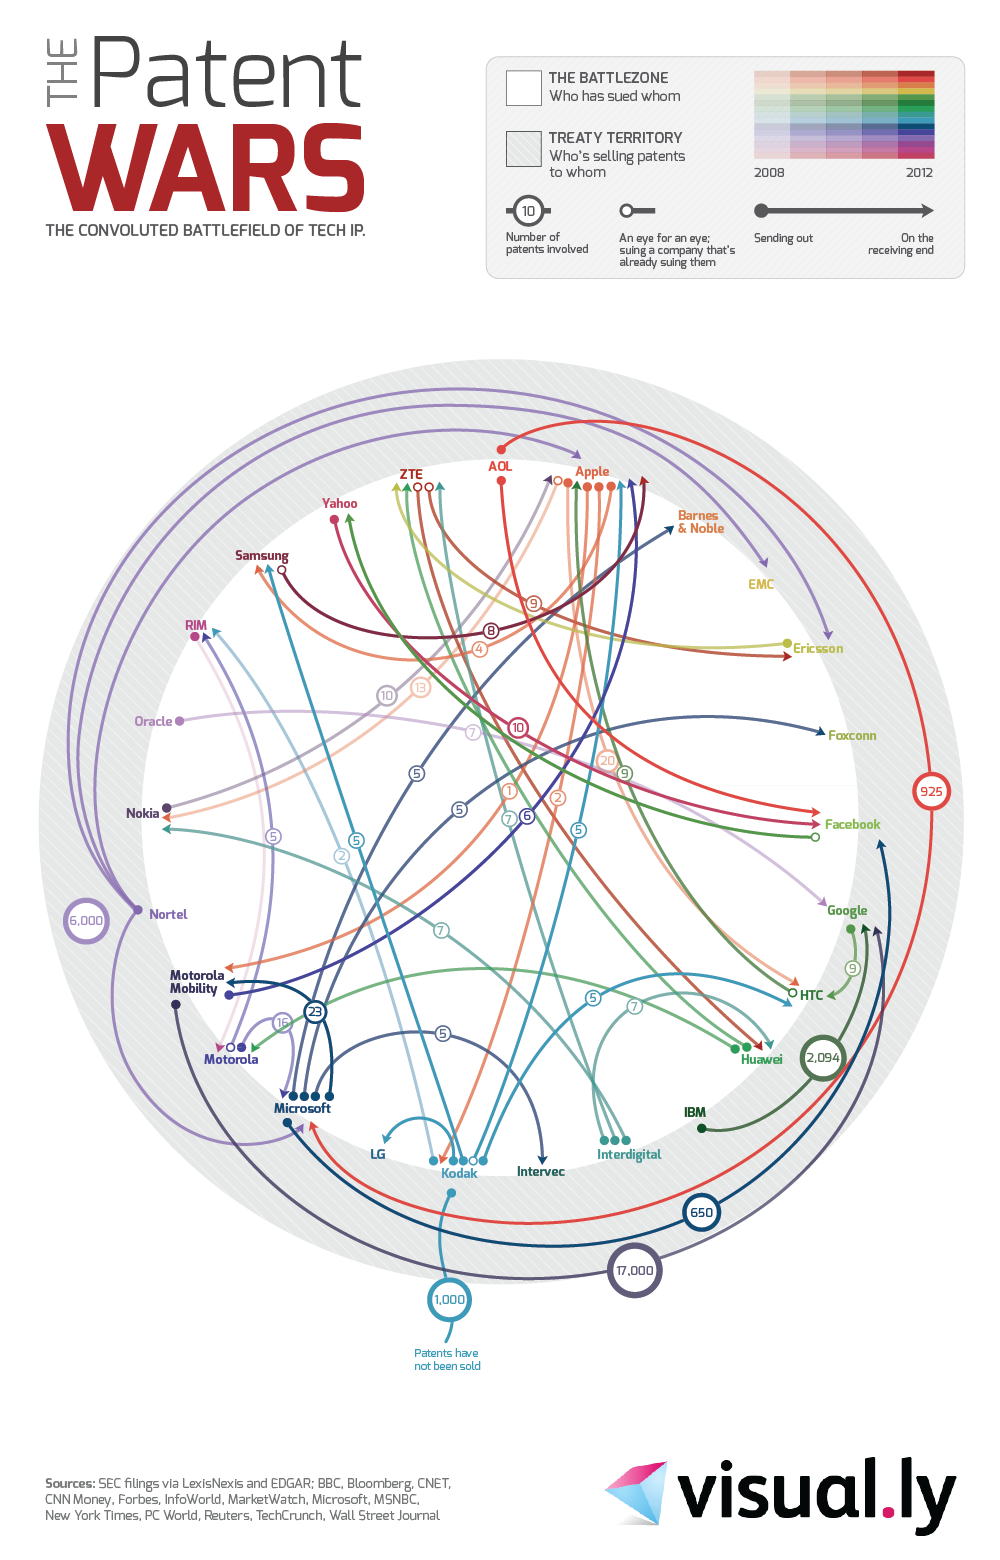
\includegraphics[scale=.442]{images/patent-wars.png}
\caption{Violations de brevet dans le domaine des smartphones}
\end{figure}

\chapter{DVD piraté vs. DVD acheté}
\label{annexe-dvd}

Source :\\
\url{http://bugbrother.blog.lemonde.fr/2010/02/22/le-fbi-menace-les-acheteurs-de-dvd/}

\newpage

\begin{figure}[H]
\center
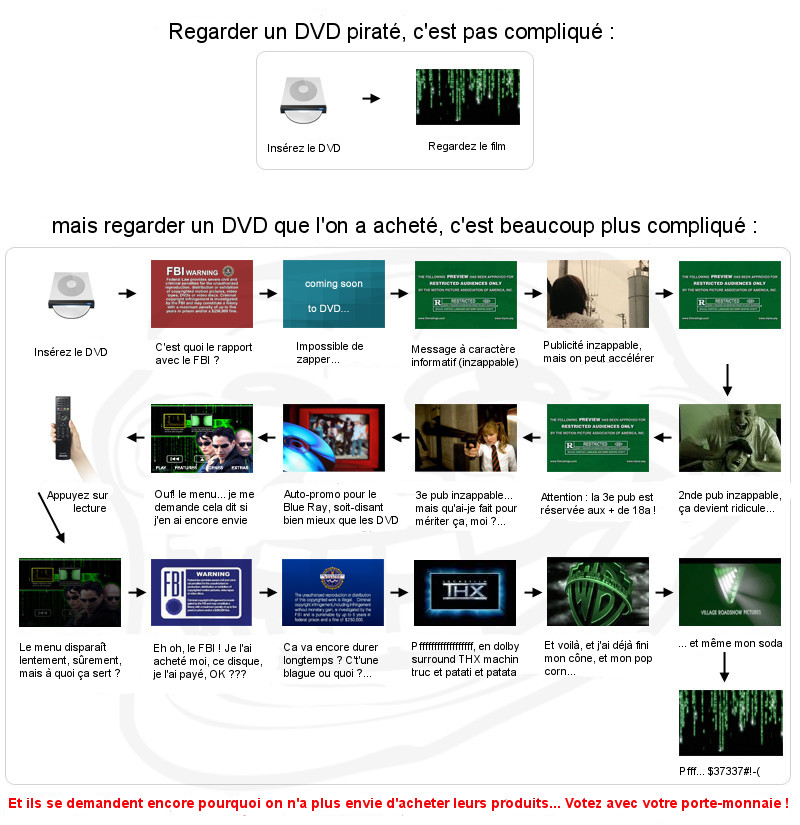
\includegraphics[scale=.602]{images/dvd-legal-dvd-illegal.jpg}
\caption{DVD piraté vs. DVD acheté}
\end{figure}

\chapter{Mon vélo, de Marcel-André Casasola Merkle}
\label{annexe-velo}

Cette traduction est une analogie qui aide à comprendre les abus et dangers du contrôle des œuvres.

Source de la traduction (licence CC-BY-SA) :\\
\url{http://reformedroitauteur.sploing.fr/\#htoc109}

Source du texte original (licence CC-BY) :\\
\url{http://www.137b.org/?p=2445}

\newpage

Je me suis acheté un vélo. Un beau modèle. Je l’ai attendu longtemps.

Aux États-Unis, ça fait déjà longtemps qu’il est sur le marché. Pas en Allemagne. Et l'importer aurait été illégal. Le mois dernier, on pouvait le louer auprès d'une grande chaîne de télé pendant une semaine et faire une virée. Ça m'a plu.

Mais à la fin de la journée, il était de nouveau verrouillé. Et je devais attendre.

Par la suite, le vélo est devenu disponible dans les arrières-cours de mon quartier pour pas un rond. Ça m'a paru un peu louche.

Mais je m'en fiche. Maintenant, j'ai mon vélo. Et il est beau.

Il est marqué jusque sur les autocollants du cadre que je ne dois pas voler ou reconstituer de vélo. Logique. Pourquoi d'ailleurs ? Je l'ai bel et bien acheté.

Avant le premier démarrage, j'ai dû appeler le fabricant et lui expliquer quels étaient les trois quartiers de la ville dans lesquels je voulais utiliser mon vélo. Lorsque je circule dans un quartier non autorisé, les freins s'enclenchent tout seul. Je n'ai rien à faire. Ça fait partie du service. Je peux alors appeler le fabricant et reconfigurer le vélo. De la sorte je circule dans toute la ville.

Si je voulais louer mon vélo, ça ne me serait pas permis. La selle envoie des petites décharges dans le corps et signifie son désaccord. C'est à la répartition des masses à l'arrière qu'elle reconnaît qui s'assoit sur le vélo. Et si ce n'est pas moi, la sonnette carillonne. Du coup, je fais attention à mon régime. Sinon mon vélo ne me reconnaît plus.

Il y a peu, j'ai voulu le repeindre. Je trouvais que le kaki faisait vieux jeu. En grande surface on m'a ri au nez. Ça serait tout à fait illégal. Est-ce que j'avais demandé au fabricant ? Il aurait sûrement dû prévoir quelque chose pour la couleur.

La ville vient de construire de nouvelles pistes cyclables et je trouvais qu'elle avait raison. Mais j'ai entendu une rumeur : Mon vélo ne peut plus rouler dessus. Les pneus sont trop minces. Ils ne passent plus sur le nouveau revêtement.

Mais une nouvelle génération arrive. Avec des chenilles. Ils seront beaucoup plus sûrs.

Et maintenant, il y a des postes de police sur les pistes. Pour contrôler qui est sur quel vélo. Et quand on perd le contact visuel avec tous les postes, le vélo éjecte son passager. Par temps de brouillard on voit souvent des hommes joncher la route comme des fruits trop mûrs.

Si on me vole mon vélo, ça peut devenir encore plus cher. Parce qu'en effet je l'ai diffusé. Le constructeur ne peut plus en vendre un directement au voleur. Et j'en suis responsable.

Tout ça m'est devenu trop périlleux. Maintenant je veux donner mon vélo à d'autres. Mais on chuchote que ce ne serait pas permis. Mon vélo ne serait qu'à moi. Je l'ai donc simplement supprimé.
